\section{Human Keypoints Estimation}
\begin{frame}{}
    \LARGE Image Segmentation: \textbf{Human Keypoints Estimation}
\end{frame}

\begin{frame}{Beyond Instance Segmentation: Human Keypoints}
    \begin{columns}
    \begin{column}{0.6\textwidth}
        \begin{itemize}
            \item Represent the pose of a human by locating a set of keypoint
            e.g. 17 keypoints:
            \item Nose
            \item Left / Right eye
            \item Left / Right earLeft / Right shoulder
            \item Left / Right elbow
            \item Left / Right wrist
        \end{itemize}
    \end{column}
    \begin{column}{0.4\textwidth}
        \begin{figure}
        \centering
        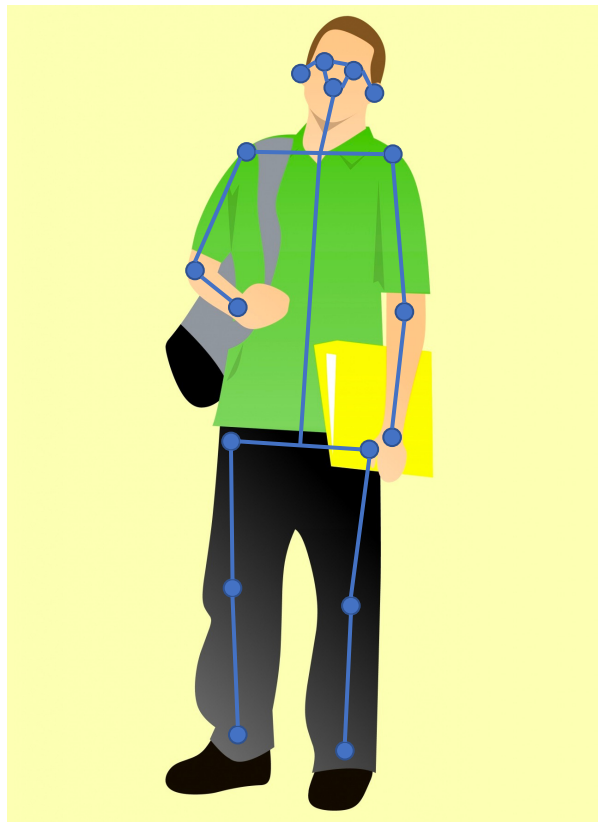
\includegraphics[width=1.0\textwidth,height=1.0\textheight,keepaspectratio]{images/segmentation/ins_12.png}
        \end{figure}
    \end{column}
    \end{columns}
\end{frame}


\begin{frame}{Mask R-CNN: Keypoint Estimation}
\only<1>{
\begin{figure}
\centering
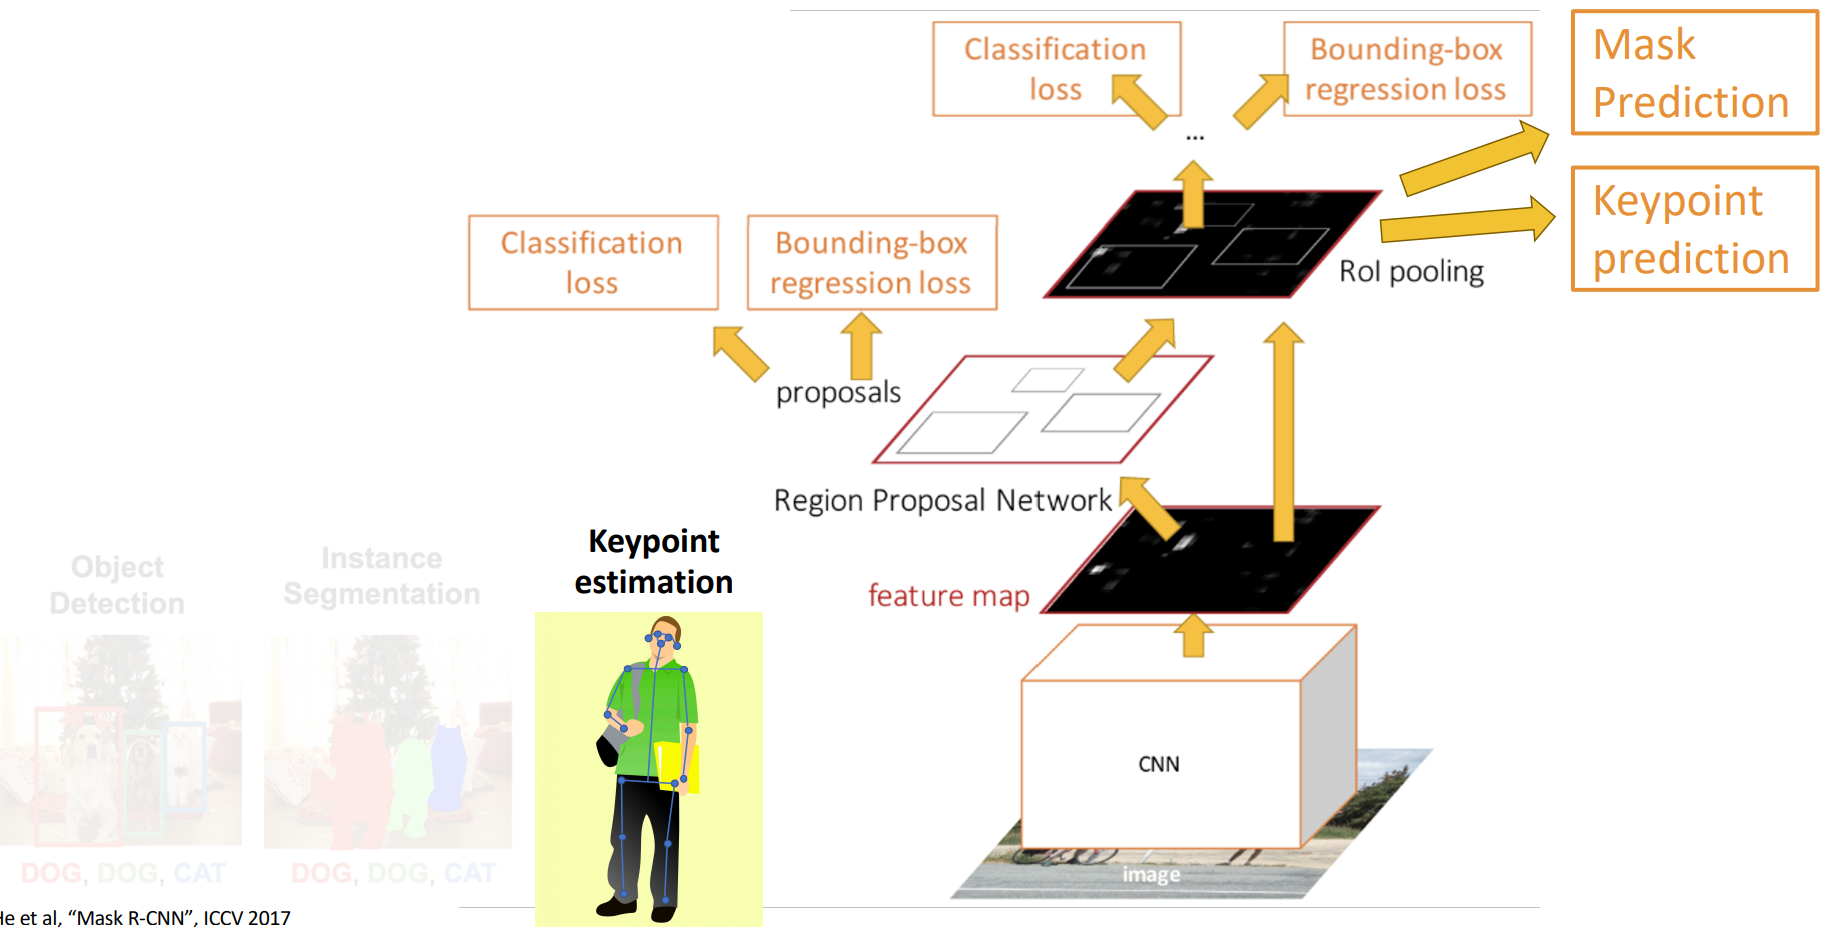
\includegraphics[width=1.0\textwidth,height=1.0\textheight,keepaspectratio]{images/segmentation/ins_13.png}
\end{figure}

}
\only<2>{
\begin{figure}
\centering
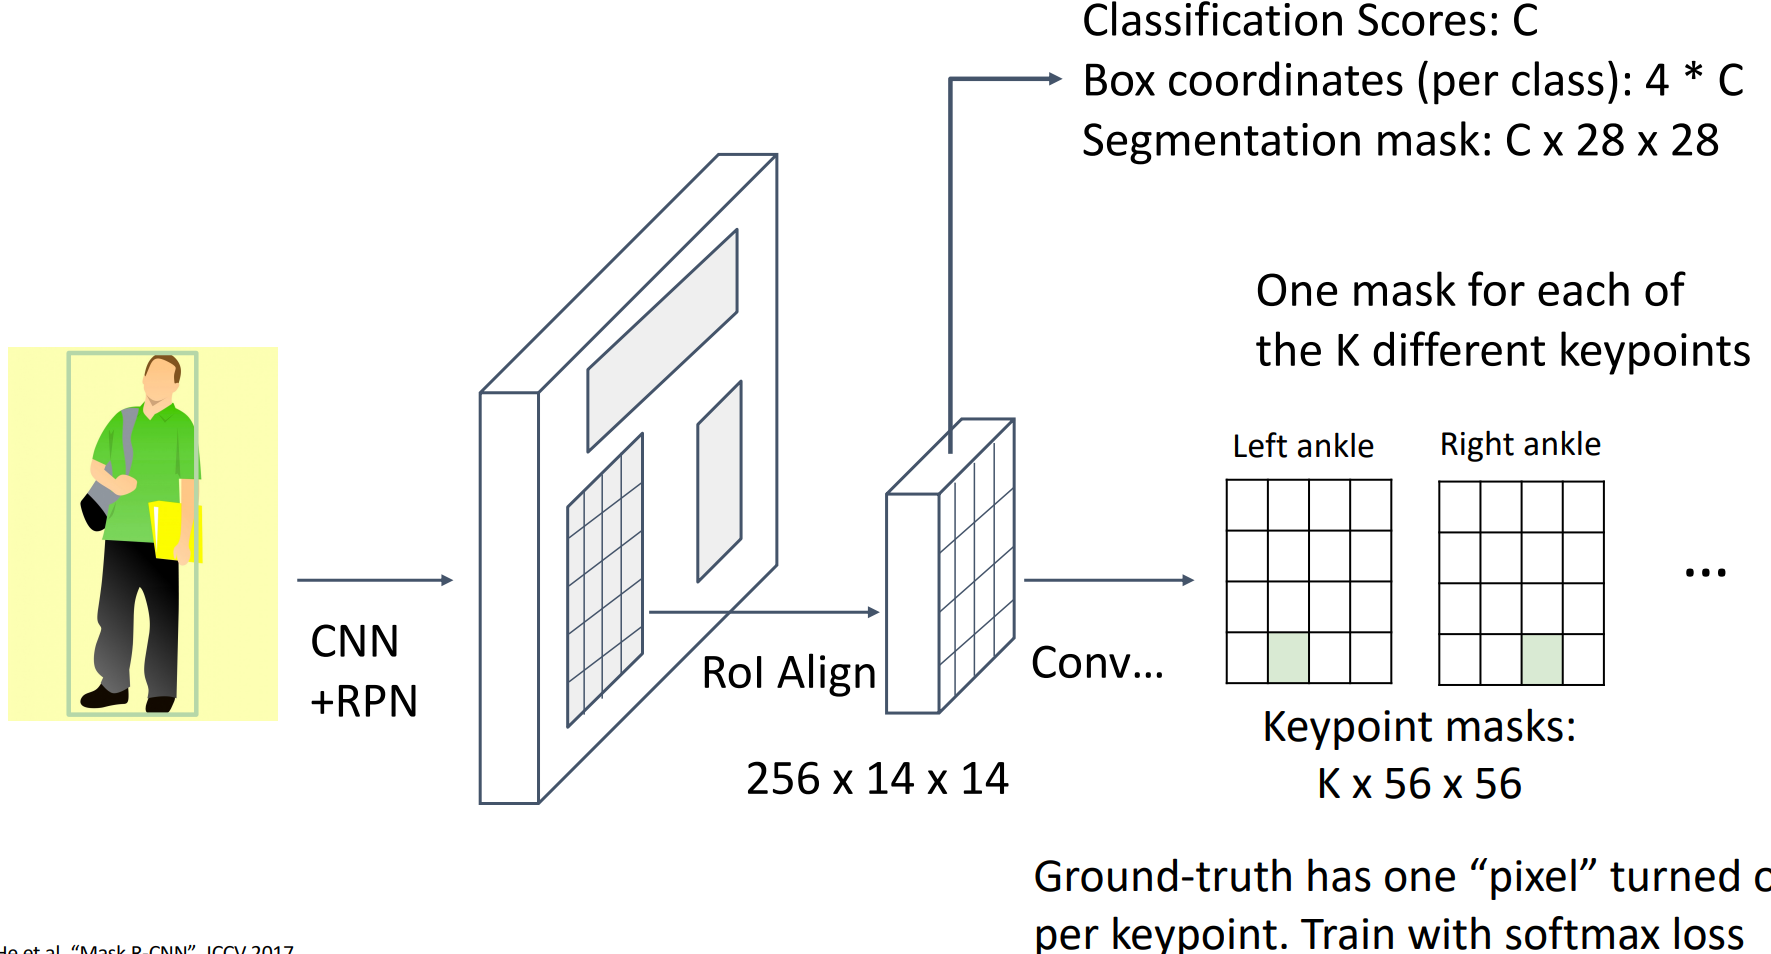
\includegraphics[width=1.0\textwidth,height=1.0\textheight,keepaspectratio]{images/segmentation/ins_14.png}
\end{figure}

}
\end{frame}